\documentclass[12pt]{article}
\usepackage[margin=2cm]{geometry}
\usepackage{amsmath}
\usepackage{amssymb} % mathbb
\usepackage{graphicx}
\usepackage{fancyvrb}

\begin{document}

\noindent
The file q4.txt defines kets, operators, and a measurement function
for simulating a four bit quantum computer.
See eigenmath.org/q.c for the program that generates q4.txt.

\bigskip
\noindent
Kets are unit vectors in $\mathbb{C}^{16}$.
The dimension is 16 because a four bit quantum computer has $2^4=16$ eigenstates.
The following basis kets are defined in q4.txt.
\begin{align*}
&|0\rangle=|0000_2\rangle=(1,0,0,0,0,0,0,0,0,0,0,0,0,0,0,0)
\\
&|1\rangle=|0001_2\rangle=(0,1,0,0,0,0,0,0,0,0,0,0,0,0,0,0)
\\
&|2\rangle=|0010_2\rangle=(0,0,1,0,0,0,0,0,0,0,0,0,0,0,0,0)
\\
&|3\rangle=|0011_2\rangle=(0,0,0,1,0,0,0,0,0,0,0,0,0,0,0,0)
\\
&\vdots
\\
&|15\rangle=|1111_2\rangle=(0,0,0,0,0,0,0,0,0,0,0,0,0,0,0,1)
\end{align*}

\noindent
Operators are $16\times16$ matrices that rotate ket vectors.
The following operators and the measurement function $M(\psi)$ are defined in q4.txt.

\bigskip
\begin{tabular}{l l}
$H_n$ & Hadamard operator on bit $n$.
\\
\\
$I$ & Identity matrix.
\\
\\
$M(\psi)$ & Measurement function (not an operator).
\\
\\
$P_{mn}(\phi)$ & Controlled phase shift, $m$ is the control bit, $n$ is the target bit, $\phi$ is the phase.
\\
\\
$Q$ & Quantum Fourier transform.
\\
\\
$R$ & Inverse quantum Fourier transform.
\\
\\
$S_{mn}$ & Swap bits $m$ and $n$.
\\
\\
$X_n$ & Pauli X (NOT) operator on bit $n$.
\\
\\
$X_{mn}$ & Controlled X (CNOT) operator, $m$ is the control bit, $n$ is the target bit.
\\
\\
$Y_n$ & Pauli Y operator on bit $n$.
\\
\\
$Z_n$ & Pauli Z operator on bit $n$.
\end{tabular}

\bigskip
\noindent
Let $\psi$ be a state of the quantum computer.
Measurement function $M(\psi)$ shows, for all $n=0\ldots15$, the probability $P_n$ of observing eigenstate $n$
given that the quantum computer is in state $\psi$.
%(Recall that the measurement process causes $\psi$ to change to the eigenstate that is observed.)
\begin{equation*}
\psi=\sum_{k=0}^{15}c_n|n\rangle,\quad|\psi|^2=1,\quad P_n=c_nc_n^*
\end{equation*}

\noindent
Quantum algorithms are expressed as sequences of operators applied
to the initial state $|0\rangle$.
The operator sequence should be read backwards, from right to left,
although the direction makes no difference mathematically.

\subsection*{Deutsch-Jozsa algorithm}
Let $f(q_0,q_1,q_2)$ be an operator ($16\times16$ matrix) that operates on $q_3$
in a manner consistent with a constant or balanced oracle.
Then the Deutsch-Jozsa algorithm for identifying $f$ is
\begin{equation*}
\psi = H_2 \; H_1 \; H_0 \; f(q_0,q_1,q_2) \; H_3 \; X_3 \; H_2 \; H_1 \; H_0 \; |0\rangle
\end{equation*}

\subsection*{Bernstein-Vazirani algorithm}
Let $f(q_0,q_1,q_2)$ be an operator ($16\times16$ matrix) that operates on $q_3$.
Then the Bernstein-Vazirani algorithm for identifying $f$ is
\begin{equation*}
\psi = H_2 \; H_1 \; H_0 \; f(q_0,q_1,q_2) \; Z_3 \; H_3 \; H_2 \; H_1 \; H_0 \; |0\rangle
\end{equation*}

\subsection*{Quantum Fourier transform}
The following circuit diagram\footnote{\tt qiskit.org/textbook/ch-algorithms/quantum-fourier-transform.html}
shows how to implement the QFT.

\begin{center}
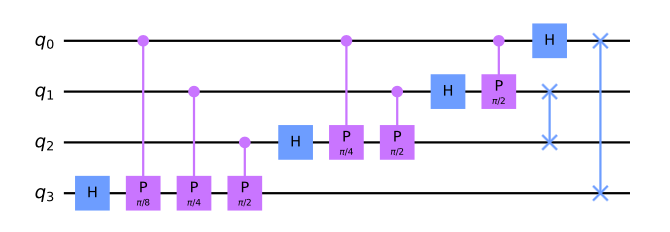
\includegraphics[scale=0.5]{qft.png}
\end{center}

\noindent
This is how the QFT operator $Q$ is defined in q4.txt.

\begin{Verbatim}
Q = dot(
S03,
S12,
H0,
P01(pi/2),
H1,
P12(pi/2),
P02(pi/4),
H2,
P23(pi/2),
P13(pi/4),
P03(pi/8),
H3)
\end{Verbatim}

\noindent
The inverse QFT operator $R$ is defined similarly except the operators appear in reverse order
and the phase shifts are negated.

\end{document}
